\subsection{Active Magnetosphere and Planetary Electrodynamics Response Experiment}

\begin{wrapfigure}{r}{0.5\textwidth} 
\vspace{-20pt}
  \begin{center}
    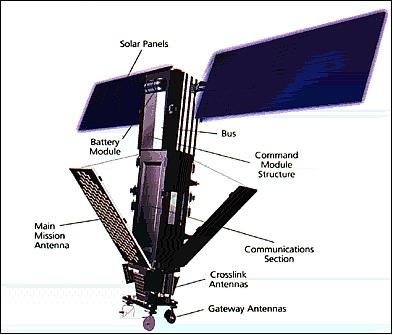
\includegraphics[width=0.4\textwidth]{Figures/Ampere/image_gallery.jpeg}
    \caption{Irridium satellite.}
    \label{fig:ACE}
  \end{center}
  \vspace{-10pt}
  \vspace{2pt}
\end{wrapfigure}

Using 66 Irridium satellites in Low Earth Orbit at $\sim 780$km altitude the Active Magnetosphere and Planetary Electrodynamics Response Experiment (AMPERE) is observing the Birkeland currents. This to create a map of the magnetic perturbation due to Field Aligned Currents. 


Something awesome


even more
